%% mle_deck.tex --- MLE I-V merged into one Beamer deck
%% Build: latexmk -pdf mle_deck.tex
\documentclass[aspectratio=169,11pt,t]{beamer}
\usefonttheme[onlymath]{serif}
\usepackage{amsmath,amssymb}
\usepackage{tikz}
\usetikzlibrary{arrows.meta,positioning}

% ------------------------------------------------------------------ look
\definecolor{navy}{RGB}{23,43,77}
\definecolor{intu}{RGB}{0,105,95}
\definecolor{flagred}{RGB}{175,30,30}
\definecolor{soft}{RGB}{233,239,247}
\definecolor{greytxt}{RGB}{110,110,110}
\setbeamercolor{structure}{fg=navy}
\setbeamercolor{frametitle}{fg=navy}
\setbeamerfont{frametitle}{series=\bfseries,size=\large}
\setbeamercolor{block title}{bg=navy,fg=white}
\setbeamercolor{block body}{bg=soft}
\setbeamercolor{block title alerted}{bg=flagred!80!black,fg=white}
\setbeamercolor{block body alerted}{bg=flagred!6}
\setbeamercolor{block title example}{bg=intu,fg=white}
\setbeamercolor{block body example}{bg=intu!7}
\setbeamertemplate{navigation symbols}{}
\setbeamertemplate{itemize items}[circle]
\setbeamertemplate{blocks}[rounded]
\setbeamertemplate{footline}{%
  \leavevmode\hbox to\paperwidth{\hspace{1em}{\tiny\color{greytxt}MLE I--V \,|\, \insertsection}\hfill
  {\tiny\color{greytxt}\insertframenumber/\inserttotalframenumber}\hspace{1em}}\vspace{4pt}}

% -------------------------------------------------------------- notation
\newcommand{\E}{\mathbb{E}}
\DeclareMathOperator{\Var}{Var}
\DeclareMathOperator{\Cov}{Cov}
\DeclareMathOperator*{\plim}{plim}
\newcommand{\cI}{\mathcal{I}}          % average (per-observation) information
\newcommand{\In}{I_{n}}                % total information
\newcommand{\cH}{\mathcal{H}}          % limiting average Hessian
\newcommand{\hth}{\hat\theta}
\newcommand{\tth}{\tilde\theta}
\newcommand{\thz}{\theta_{0}}
\newcommand{\asim}{\overset{a}{\sim}}
\newcommand{\aeq}{\overset{a}{=}}
\newcommand{\dto}{\overset{d}{\longrightarrow}}

% --------------------------------------------------------------- helpers
\newcommand{\why}[1]{\qquad\text{\footnotesize\color{greytxt}[#1]}}
\newcommand{\intuition}[1]{\par\vfill
  {\color{intu}\rule{\linewidth}{0.4pt}}\par\vspace{1pt}
  {\small\color{intu}\textbf{Intuition.}\ #1}\par\vspace{2pt}}
\newcommand{\flag}[1]{\par\smallskip{\scriptsize\color{flagred}\textbf{Check:}\ #1}\par}
\newcommand{\bridge}[3]{%
  \begin{frame}{#1}
  \vspace{4pt}
  \begin{block}{Where we are}#2\end{block}
  \begin{exampleblock}{What's next}#3\end{exampleblock}
  \end{frame}}

\title{Maximum Likelihood: Estimation and Testing}
\subtitle{MLE I--V as one connected story}
\author{Econometrics I --- class notes}
\date{}

\begin{document}

% =====================================================================
\begin{frame}[plain,c]
\titlepage
\end{frame}

% ---------------------------------------------------------------------
\section{Roadmap}
\begin{frame}{Roadmap: one chain from the likelihood to the tests}
{\centering
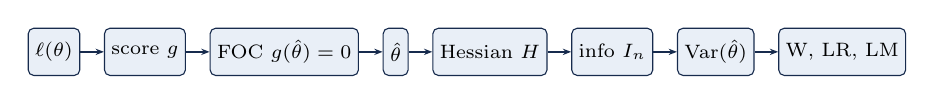
\begin{tikzpicture}[
  box/.style={draw=navy,fill=soft,rounded corners=2pt,inner sep=2.5pt,font=\scriptsize,minimum height=6mm},
  arr/.style={-{Stealth[length=3pt]},navy,thick}]
 \node[box] (l) {$\ell(\theta)$};
 \node[box,right=3mm of l] (g) {score $g$};
 \node[box,right=3mm of g] (f) {FOC $g(\hth)=0$};
 \node[box,right=3mm of f] (t) {$\hth$};
 \node[box,right=3mm of t] (h) {Hessian $H$};
 \node[box,right=3mm of h] (i) {info $\In$};
 \node[box,right=3mm of i] (v) {$\Var(\hth)$};
 \node[box,right=3mm of v] (w) {W, LR, LM};
 \foreach \a/\b in {l/g,g/f,f/t,t/h,h/i,i/v,v/w} \draw[arr] (\a) -- (\b);
\end{tikzpicture}\par}

\vspace{6pt}
\footnotesize
\begin{columns}[T,onlytextwidth]
\begin{column}{0.5\textwidth}
\begin{enumerate}
 \item \textbf{Why ML?} When least squares breaks down.
 \item \textbf{Building blocks:} score, Hessian, information.
 \item \textbf{Distribution of $\hth$:} how precise is it?
 \item \textbf{Estimating $\Var(\hth)$} in practice.
 \item \textbf{Worked example:} normal linear model, ML $=$ OLS.
 \item \textbf{When ML $\neq$ LS:} Jacobian terms.
\end{enumerate}
\end{column}
\begin{column}{0.5\textwidth}
\begin{enumerate}\setcounter{enumi}{6}
 \item \textbf{Testing principles:} W, LR, LM.
 \item \textbf{LM from restricted ML}: why it is $\chi^{2}_{r}$.
 \item \textbf{W $\ge$ LR $\ge$ LM} in the linear model.
 \item \textbf{Hausman}: comparing two estimators.
 \item \textbf{LM by regression}: $nR^{2}$ and AR(1) errors.
\end{enumerate}
\end{column}
\end{columns}
\intuition{Each section answers the question the previous one leaves open. Red ``Check'' lines mark places where the deck departs from, or corrects, the handouts.}
\end{frame}

% ---------------------------------------------------------------------
\begin{frame}{Notation used on every slide}
\footnotesize
\begin{columns}[T,onlytextwidth]
\begin{column}{0.52\textwidth}
\renewcommand{\arraystretch}{1.2}\setlength{\tabcolsep}{3pt}
\begin{tabular}{@{}l@{\ \ }l@{}}
 $\theta$ ($k\times1$), $\thz$ & parameters; true value\\
 $\hth$, $\tth$ & unrestricted / restricted MLE\\
 $\ell_{t}(\theta)=\log f(y_{t};\theta)$ & contribution of obs.\ $t$\\
 $\ell(\theta)=\sum_{t=1}^{n}\ell_{t}(\theta)$ & log-likelihood\\
 $g(\theta)=\partial\ell/\partial\theta$ & score ($k\times1$)\\
 $G(\theta)$, $G_{ti}=\partial\ell_{t}/\partial\theta_{i}$ & CG matrix ($n\times k$), $g=G'\iota$\\
 $H(\theta)=\partial^{2}\ell/\partial\theta\,\partial\theta'$ & Hessian ($k\times k$)\\
 $\In(\theta)=\E[g g']$ & \textbf{total} information ($k\times k$)\\
 $\cI(\theta)=\lim \In/n$ & \textbf{average} information\\
 $\cH(\theta)=\plim H/n$ & average Hessian
\end{tabular}
\end{column}
\begin{column}{0.46\textwidth}
\renewcommand{\arraystretch}{1.2}
\begin{tabular}{@{}l@{\ \ }l@{}}
 $r(\theta)=0$ & $r$ restrictions under $H_{0}$\\
 $R(\theta)=\partial r/\partial\theta'$ & $r\times k$\\
 $\lambda$ & multipliers ($r\times1$)\\
 $\Lambda=L(\theta_{0})/L(\theta_{1})$ & likelihood ratio\\
 $\iota=(1,\dots,1)'$ & $n\times1$\\
 $\asim$ / $\aeq$ & asympt.\ distributed / equal
\end{tabular}

\vspace{6pt}
\textbf{Key scaling:} $\In=n\,\cI$, so
\[ \Var(\hth)\approx\In^{-1}=\tfrac1n\cI^{-1}. \]
\end{column}
\end{columns}
\flag{the handouts mix scalings: MLE I--III use $\cI$ for the \emph{average} information; MLE IV (E4) and MLE V write $\cI$ for the \emph{total} ($X'X/\sigma^{2}$, $n/2\sigma^{4}$). Here: $\In$ total, $\cI$ average. Renamed: $T\to n$ (MLE III), $L\to\ell$ for the log-likelihood (MLE V), LR ratio $\lambda\to\Lambda$, Box--Cox $\lambda\to\kappa$, Hausman weight $\lambda\to w$.}
\end{frame}

% =====================================================================
\section{1 Why ML?}

\begin{frame}{Least squares needs ``$y=$ regression $+$ error''; some models are not}
\[ y_{t}^{\gamma}=\beta_{0}+\beta_{1}x_{t}+u_{t},\qquad u_{t}\sim\text{IID}(0,\sigma^{2}). \]
\begin{itemize}
 \item $\gamma$ known: an ordinary regression of $y_{t}^{\gamma}$ on $x_{t}$.
 \item $\gamma$ unknown: minimise $\ \mathrm{SSR}(\beta,\gamma)=\sum_{t}\bigl(y_{t}^{\gamma}-\beta_{0}-\beta_{1}x_{t}\bigr)^{2}$?
\end{itemize}
The SSR can be driven to zero \emph{without using the data}:
\begin{align*}
 \gamma=0,\ \beta_{0}=1,\ \beta_{1}=0:&\quad y_{t}^{0}-1=0\ \text{for every }t \;\Rightarrow\; \mathrm{SSR}=0;\\
 \gamma\to-\infty,\ \beta_{0}=\beta_{1}=0:&\quad y_{t}^{\gamma}\to0\ \text{if all } y_{t}>1 \;\Rightarrow\; \mathrm{SSR}\to0.
\end{align*}
\intuition{SSR measures the fit of the \emph{transformed} $y$. By changing $\gamma$ it changes what is being fitted. We need a criterion that charges for the transformation (that is the Jacobian, Section 6).}
\end{frame}

\begin{frame}{ML picks the $\theta$ under which the observed sample is most probable}
\begin{align*}
 L(\theta)&=\prod_{t=1}^{n}f(y_{t};\theta) \why{independent observations: joint density $=$ product}\\
 \ell(\theta)=\log L(\theta)&=\sum_{t=1}^{n}\ell_{t}(\theta) \why{$\log$ turns the product into a sum}
\end{align*}
$\log$ is strictly increasing, so $L$ and $\ell$ have the same maximiser. Two definitions:
\begin{itemize}
 \item \textbf{Type 1:} $\hth$ is a global maximiser, $\ell(\hth)\ge\ell(\theta^{*})$ for all $\theta^{*}\in\Theta$.
 \item \textbf{Type 2:} $\hth$ solves the likelihood equations $g(\hth)=0$ (used for the asymptotics).
\end{itemize}
\intuition{Read $L(\theta)$ as ``how surprised would I be to see this sample if $\theta$ were true''; ML picks the least surprising $\theta$.}
\end{frame}

\begin{frame}{First example: the exponential distribution gives $\hth=1/\bar y$}
Density $f(y_{t};\theta)=\theta e^{-\theta y_{t}}$, $y_{t}>0$, $\theta>0$.
\begin{align*}
 \ell(\theta)&=\sum_{t}\bigl(\log\theta-\theta y_{t}\bigr)=n\log\theta-\theta\textstyle\sum_{t}y_{t}
   \why{log of each density, summed}\\
 g(\theta)&=\frac{n}{\theta}-\textstyle\sum_{t}y_{t}
   \why{differentiate}\\
 g(\hth)=0\ &\Longrightarrow\ \hth=\frac{n}{\sum_{t}y_{t}}=\frac1{\bar y}
   \why{first-order condition}\\
 H(\theta)&=-\frac{n}{\theta^{2}}<0
   \why{so $\hth$ is a maximum}
\end{align*}
\intuition{$\E(y_{t})=1/\theta$, so ML sets the model mean equal to the sample mean here. We reuse this model to check every link of the chain (Section 3).}
\end{frame}

\begin{frame}{Invariance: reparametrising does not change ML, but makes it biased}
Let $\phi=\eta(\theta)$ be one-to-one and write $\ell^{*}(\phi)=\ell\bigl(\eta^{-1}(\phi)\bigr)$. Then for every $\theta^{*}$
\[ \ell^{*}\bigl(\eta(\hth)\bigr)=\ell(\hth)\ \ge\ \ell(\theta^{*})=\ell^{*}\bigl(\eta(\theta^{*})\bigr)
   \quad\Longrightarrow\quad \hat\phi=\eta(\hth). \]
\textbf{Consequence: bias.} Even if $\E(\hth)=\theta$, for nonlinear $\eta$ (Jensen)
\[ \E(\hat\phi)=\E\bigl(\eta(\hth)\bigr)\neq\eta\bigl(\E\hth\bigr)=\phi . \]
\emph{Example (added).} Exponential model: the mean $\mu=1/\theta$ has $\hat\mu=\bar y$, which is unbiased.
Then $\hth=1/\bar y$ has $\E(\hth)=\tfrac{n}{n-1}\theta>\theta$.
\intuition{ML cannot be unbiased in every parametrisation at once. The bias disappears as $n\to\infty$, so the parametrisation only matters in small samples.}
\end{frame}

\bridge{Open question: $\hth$ is random. How precise is it?}
{We have a definition ($g(\hth)=0$) and examples. We know $\hth$ is invariant but generally biased.}
{To find the distribution of $\hth$ we need the derivatives of $\ell$, organised as vectors and matrices: score, CG matrix, Hessian, information.}

% =====================================================================
\section{2 Building blocks}

\begin{frame}{The score stacks $k$ slopes, and each slope is a sum over observations}
\[ \underset{k\times1}{g(\theta)}=\frac{\partial\ell(\theta)}{\partial\theta}=
 \begin{bmatrix}\partial\ell/\partial\theta_{1}\\ \partial\ell/\partial\theta_{2}\\ \vdots\\ \partial\ell/\partial\theta_{k}\end{bmatrix},
 \qquad
 \text{typical element}\quad g_{i}(\theta)=\sum_{t=1}^{n}\frac{\partial\ell_{t}(\theta)}{\partial\theta_{i}} . \]
\begin{itemize}
 \item The likelihood equations $g(\hth)=0$ are $k$ equations in the $k$ unknowns $\hth$.
 \item Each $g_{i}$ is a sum of $n$ terms, so laws of large numbers and CLTs apply to it.
\end{itemize}
\intuition{$g$ is the slope of the log-likelihood in each direction. At the top of the hill every slope is zero.}
\end{frame}

\begin{frame}{The CG matrix keeps the score's contribution from each observation}
\[ \underset{n\times k}{G(\theta)}=
 \begin{bmatrix}
  \partial\ell_{1}/\partial\theta_{1} & \cdots & \partial\ell_{1}/\partial\theta_{k}\\
  \vdots & \ddots & \vdots\\
  \partial\ell_{n}/\partial\theta_{1} & \cdots & \partial\ell_{n}/\partial\theta_{k}
 \end{bmatrix},
 \qquad G_{ti}=\frac{\partial\ell_{t}}{\partial\theta_{i}},\qquad
 \text{row } t:\ \underset{1\times k}{G_{t}}=\frac{\partial\ell_{t}}{\partial\theta'} . \]
Summing the rows gives the score:
\[ g(\theta)=G'(\theta)\,\iota,
   \qquad\text{since}\quad [G'\iota]_{i}=\sum_{t=1}^{n}G_{ti}\cdot1=g_{i}. \]
\intuition{$G$ is like a ``data matrix'' of score contributions. Its cross-product $G'G$ will estimate the information (OPG, Section 4), and regressions on $G$ give LM tests.}
\end{frame}

\begin{frame}{The Hessian collects all $k^{2}$ second derivatives}
\[ \underset{k\times k}{H(\theta)}=\frac{\partial^{2}\ell}{\partial\theta\,\partial\theta'}=
 \begin{bmatrix}
  \dfrac{\partial^{2}\ell}{\partial\theta_{1}^{2}} & \cdots & \dfrac{\partial^{2}\ell}{\partial\theta_{1}\partial\theta_{k}}\\[8pt]
  \vdots & \ddots & \vdots\\
  \dfrac{\partial^{2}\ell}{\partial\theta_{k}\partial\theta_{1}} & \cdots & \dfrac{\partial^{2}\ell}{\partial\theta_{k}^{2}}
 \end{bmatrix},
 \qquad H_{ij}=\sum_{t=1}^{n}\frac{\partial^{2}\ell_{t}}{\partial\theta_{i}\,\partial\theta_{j}} . \]
\begin{itemize}
 \item Symmetric ($H_{ij}=H_{ji}$). Negative definite at a regular maximum.
 \item Average version: $\cH(\theta)=\plim\frac1nH(\theta)$, which is $O(1)$, while $H$ itself is $O(n)$.
\end{itemize}
\intuition{$H$ is the curvature of $\ell$. A sharply curved peak means the data pin $\theta$ down well, so the variance is small.}
\end{frame}

\begin{frame}{The information matrix is the expected outer product of the score}
Per observation (note $G_{t}'G_{t}$: $(k\times1)(1\times k)=k\times k$):
\[ \underset{k\times k}{I_{t}(\theta)}=\E\bigl[G_{t}'G_{t}\bigr],\qquad [I_{t}]_{ij}=\E\bigl[G_{ti}\,G_{tj}\bigr]. \]
Whole sample, total and average:
\[ \In(\theta)=\sum_{t=1}^{n}I_{t}=\E\bigl[G'G\bigr]=
 \begin{bmatrix}
  \sum_{t}\E[G_{t1}^{2}] & \cdots & \sum_{t}\E[G_{t1}G_{tk}]\\
  \vdots & \ddots & \vdots\\
  \sum_{t}\E[G_{tk}G_{t1}] & \cdots & \sum_{t}\E[G_{tk}^{2}]
 \end{bmatrix}. \]
Average: $\cI(\theta)=\lim_{n\to\infty}\In/n$. Orders: $\In=O(n)$ and $\cI=O(1)$. Both are symmetric and p.s.d.
\flag{MLE I writes $I_{t}=\E(G_{t}G_{t}')$. For a $1\times k$ row that product is a scalar; the $k\times k$ matrix is $\E(G_{t}'G_{t})$.}
\intuition{Information adds up across independent observations, so it grows like $n$ and the variance shrinks like $1/n$.}
\end{frame}

\bridge{Open question: what is the distribution of $\hth-\thz$?}
{We have $g$ ($k\times1$), $G$ ($n\times k$), $H$ ($k\times k$) and $\In=\E(G'G)$ ($k\times k$).}
{Linearise the first-order condition around $\thz$. Five steps give $\sqrt n(\hth-\thz)\dto N(0,\cI^{-1})$.}

% =====================================================================
\section{3 Distribution of the MLE}

\begin{frame}{Step 1: a Taylor expansion turns the FOC into a formula for $\hth-\thz$}
Consistency, $\plim\hth=\thz$, is assumed (it holds under regularity conditions; the proof is omitted).
\begin{align*}
 0=g(\hth)&=g(\thz)+H(\bar\theta)\,(\hth-\thz)
   \why{mean-value expansion, $\bar\theta$ between $\hth$ and $\thz$}\\
 \hth-\thz&=-H(\bar\theta)^{-1}\,g(\thz)
   \why{solve for $\hth-\thz$}
\end{align*}
\intuition{This is one Newton step. Estimation error $=-$(curvature)$^{-1}\times$(slope at the truth).}
\end{frame}

\begin{frame}{Step 2: rescale so every factor has a limit}
Multiply by $\sqrt n$ and split the powers of $n$:
\[ \sqrt n\,(\hth-\thz)=-\Bigl(\frac{H(\bar\theta)}{n}\Bigr)^{-1}\frac{g(\thz)}{\sqrt n}
   \why{check: $n\cdot n^{-1/2}=\sqrt n$} \]
\begin{itemize}
 \item $\frac1nH(\bar\theta)$ is an average of $n$ terms, so by a LLN it tends to $\cH(\thz)$
       (also using that $\bar\theta$ is squeezed between $\hth$ and $\thz$, so $\bar\theta\to\thz$).
 \item $\frac1{\sqrt n}g(\thz)$ is a sum of $n$ terms over $\sqrt n$, which is CLT-sized: $O_{p}(1)$.
\end{itemize}
\[ \boxed{\ \sqrt n\,(\hth-\thz)\ \aeq\ -\cH(\thz)^{-1}\,\frac{g(\thz)}{\sqrt n}\ } \]
\intuition{All the randomness is now in one vector, the scaled score at the truth. We need its mean (Step 3) and its variance (Step 4).}
\end{frame}

\begin{frame}{Step 3: the score has mean zero at the true $\theta$}
For each observation $t$ and parameter $i$, with $L_{t}=f(y_{t};\theta)$ the density:
\begin{align*}
 \E\Bigl[\frac{\partial\ell_{t}}{\partial\theta_{i}}\Big|_{\thz}\Bigr]
 &=\int\frac{1}{L_{t}}\frac{\partial L_{t}}{\partial\theta_{i}}\;L_{t}\,dy_{t}
   \why{$\partial\log L_{t}=\partial L_{t}/L_{t}$; expectation under the density $L_{t}(\thz)$}\\
 &=\int\frac{\partial L_{t}}{\partial\theta_{i}}\,dy_{t}
   \why{the $L_{t}$'s cancel}\\
 &=\frac{\partial}{\partial\theta_{i}}\int L_{t}\,dy_{t}
   \why{regularity: swap $\partial$ and $\int$}\\
 &=\frac{\partial}{\partial\theta_{i}}\,1=0
   \why{a density integrates to one for every $\theta$}
\end{align*}
Hence $\E[G_{ti}(\thz)]=0$ for all $t,i$, and $\E[g(\thz)/\sqrt n]=0$.
\intuition{At the truth there is no systematic direction in which moving $\theta$ raises the likelihood.}
\end{frame}

\begin{frame}{Step 4: the variance of the score is the information matrix}
Mean zero, so the variance is $\frac1n\E[gg']$. Its $(i,j)$ element is a double sum over pairs $(t,s)$:
\begin{align*}
 \tfrac1n\E\bigl[g_{i}g_{j}\bigr]
 &=\tfrac1n\E\Bigl[\Bigl(\textstyle\sum_{t}G_{ti}\Bigr)\Bigl(\sum_{s}G_{sj}\Bigr)\Bigr]
  =\tfrac1n\textstyle\sum_{t}\sum_{s}\E\bigl[G_{ti}G_{sj}\bigr]\\
 t\neq s:\quad \E[G_{ti}G_{sj}]&=\E[G_{ti}]\,\E[G_{sj}]=0\cdot0
   \why{independence, then Step 3}\\
 \Longrightarrow\quad \tfrac1n\E\bigl[g_{i}g_{j}\bigr]&=\tfrac1n\textstyle\sum_{t}\E\bigl[G_{ti}G_{tj}\bigr]=\tfrac1n\bigl[\E(G'G)\bigr]_{ij}
   \why{only $t=s$ survives}
\end{align*}
\[ \Var\Bigl(\frac{g(\thz)}{\sqrt n}\Bigr)=\frac1n\E\bigl[gg'\bigr]=\frac1n\E\bigl[G'G\bigr]=\frac{\In(\thz)}{n}\ \longrightarrow\ \cI(\thz). \]
\intuition{Of the $n^{2}$ cross products only the $n$ ``own'' terms have nonzero mean, which is why the information is additive.}
\end{frame}

\begin{frame}{Step 5: a CLT and a linear map give a sandwich variance}
\begin{align*}
 \frac{g(\thz)}{\sqrt n}&\ \dto\ N\bigl(0,\cI\bigr)
   \why{CLT: scaled sum of independent, mean-zero terms}\\
 \sqrt n(\hth-\thz)&\ \aeq\ A\,\frac{g(\thz)}{\sqrt n},\qquad A=-\cH^{-1}
   \why{Step 2}\\
 \Var\bigl(\sqrt n(\hth-\thz)\bigr)&=A\,\cI\,A'=\cH^{-1}\,\cI\,\cH^{-1}
   \why{$\Var(Az)=A\Var(z)A'$, and $\cH$ is symmetric}
\end{align*}
\[ \boxed{\ \sqrt n\,(\hth-\thz)\ \dto\ N\bigl(0,\ \cH^{-1}\cI\,\cH^{-1}\bigr)\ } \]
\intuition{So far we have only used independence and regularity, not that the model is correct. That is why the sandwich is the ``robust'' form.}
\end{frame}

\begin{frame}{Information matrix equality: $\cH=-\cI$, but only if the model is right}
Quotient rule on $\partial\ell_{t}/\partial\theta_{i}=\frac{1}{L_{t}}\partial L_{t}/\partial\theta_{i}$:
\[ \frac{\partial^{2}\ell_{t}}{\partial\theta_{i}\partial\theta_{j}}
 =\frac{1}{L_{t}}\frac{\partial^{2}L_{t}}{\partial\theta_{i}\partial\theta_{j}}
 -\frac{\partial\ell_{t}}{\partial\theta_{i}}\frac{\partial\ell_{t}}{\partial\theta_{j}} . \]
Move the outer product to the left and look at the \textbf{gap}:
\[ \underbrace{\E\Bigl[\frac{\partial^{2}\ell_{t}}{\partial\theta_{i}\partial\theta_{j}}\Bigr]+\E\bigl[G_{ti}G_{tj}\bigr]}_{\text{gap}}
 =\E\Bigl[\frac{1}{L_{t}}\frac{\partial^{2}L_{t}}{\partial\theta_{i}\partial\theta_{j}}\Bigr]
 =\int\frac{\partial^{2}L_{t}}{\partial\theta_{i}\partial\theta_{j}}dy_{t}
 =\frac{\partial^{2}}{\partial\theta_{i}\partial\theta_{j}}\!\int\! L_{t}\,dy_{t}=0 . \]
The second ``$=$'' needs the expectation to be taken under $L_{t}(\thz)$ itself, i.e.\ the \textbf{true density is the model density}. If the model is misspecified the gap is not zero.
\[ \text{correct model}\ \Longrightarrow\ \cH(\thz)=-\cI(\thz). \]
\intuition{Two measures of how informative the data are agree: the curvature of $\ell$ ($-\cH$) and the variability of its slope ($\cI$). They agree only if the model is right.}
\end{frame}

\begin{frame}{With a correct model the three variance formulas collapse into one}
Substitute $\cH=-\cI$ into the sandwich:
\[ \underbrace{\cH^{-1}\cI\,\cH^{-1}}_{\text{(A) sandwich}}
 =(-\cI)^{-1}\,\cI\,(-\cI)^{-1}
 =\underbrace{\cI^{-1}}_{\text{(C)}}
 =\underbrace{-\cH^{-1}}_{\text{(B)}} . \]
\[ \boxed{\ \sqrt n(\hth-\thz)\ \dto\ N\bigl(0,\cI(\thz)^{-1}\bigr),
   \qquad\text{i.e.}\qquad \hth\ \asim\ N\bigl(\thz,\ \In(\thz)^{-1}\bigr)\ } \]
\begin{itemize}
 \item (A) is valid without the IM equality, so use it when the model is in doubt.
 \item (B) and (C) need the model to be correctly specified.
\end{itemize}
\intuition{``Inverse information'' is the answer when the model is right; the sandwich is the safe answer when it may not be.}
\end{frame}

\begin{frame}{Check the whole chain on the exponential model (added)}
$\ell_{t}=\log\theta-\theta y_{t}$, and $\E(y_{t})=1/\theta$, $\Var(y_{t})=1/\theta^{2}$.
\begin{align*}
 \text{score contribution:}\quad & G_{t}=\tfrac1\theta-y_{t}\\
 \text{mean zero:}\quad & \E[G_{t}]=\tfrac1\theta-\tfrac1\theta=0 \why{Step 3 holds}\\
 \text{information:}\quad & I_{t}=\E\bigl[(\tfrac1\theta-y_{t})^{2}\bigr]=\Var(y_{t})=\tfrac1{\theta^{2}}\\
 \text{minus expected Hessian:}\quad & -\E\bigl[\partial^{2}\ell_{t}/\partial\theta^{2}\bigr]=\tfrac{1}{\theta^{2}}=I_{t} \why{IM equality holds}\\
 \text{variance:}\quad & \Var(\hth)\approx\In^{-1}=\tfrac{\theta^{2}}{n},\qquad
 \widehat{\Var}(\hth)=\tfrac{\hth^{2}}{n}=\tfrac{1}{n\bar y^{2}}
\end{align*}
\intuition{Every abstract step can be checked by hand in a one-parameter model. Do this when a general formula looks suspicious.}
\end{frame}

\begin{frame}{Cram\'er--Rao: ML reaches the efficiency bound $\In^{-1}$ asymptotically}
For any unbiased estimator $\check\theta$, the \textbf{gap} is positive semidefinite:
\[ \Var(\check\theta)-\In(\thz)^{-1}\ \succeq\ 0 . \]
ML's asymptotic variance is $\In^{-1}=\frac1n\cI^{-1}$, so for ML the gap tends to zero:
\begin{itemize}
 \item ML is \textbf{asymptotically efficient}: no consistent, asymptotically unbiased estimator (linear or not) does better.
 \item This is asymptotic only. In finite samples ML is generally biased (invariance) and need not reach the bound.
\end{itemize}
\flag{MLE II writes the bound as $\cI^{-1}(\thz)$. With $\cI$ the \emph{average} information the bound for $\Var(\check\theta)$ is $\In^{-1}=(n\cI)^{-1}$.}
\intuition{The gap is the information an estimator wastes. ML wastes none in the limit.}
\end{frame}

\bridge{Open question: $\cI(\thz)$ is unknown. How do we estimate $\Var(\hth)$?}
{$\hth\asim N(\thz,\In^{-1})$ under a correct model, or the sandwich otherwise. ML is asymptotically efficient.}
{Replace $\thz$ by $\hth$, and the expectation by one of three sample counterparts. One of them comes out of an OLS regression.}

% =====================================================================
\section{4 Estimating the variance}

\begin{frame}{Three consistent estimators of $\Var(\hth)$, equal under a correct model}
\renewcommand{\arraystretch}{1.5}
\small
\begin{tabular}{@{}l l p{0.5\textwidth}@{}}
 & \textbf{estimator} & \textbf{pros / cons}\\ \hline
 (I) information & $\In(\hth)^{-1}$ & best in principle; expectations often impossible analytically\\
 (II) Hessian & $\bigl[-H(\hth)\bigr]^{-1}$ & p.d.\ at a regular max; second derivatives can be tedious\\
 (III) OPG & $\bigl[G(\hth)'G(\hth)\bigr]^{-1}$ & first derivatives only; uses $\E(gg')=\E(G'G)$ (independence)\\
 sandwich & $H^{-1}(G'G)H^{-1}\big|_{\hth}$ & form (A); valid without the IM equality (\emph{added})
\end{tabular}

\vspace{6pt}
Numerical second derivatives are an option for (II), but they can be very unreliable.
\intuition{Each estimator plugs a sample version of $\cI$ or $\cH$ into the formulas of Section 3.}
\end{frame}

\begin{frame}{The OPG regression: regress a column of ones on $\hat G$}
\[ \iota=\hat G\,b+\text{residuals},\qquad \hat G=G(\hth). \]
\begin{align*}
 \hat b&=(\hat G'\hat G)^{-1}\hat G'\iota=(\hat G'\hat G)^{-1}\hat g
   \why{$\hat G'\iota=\hat g$}\\
 &=0 \why{$\hat g=g(\hth)=0$: $\hth$ solves the likelihood equations}\\
 \text{residuals}&=\iota-\hat G\hat b=\iota,\qquad s^{2}=\tfrac{1}{n-k}\textstyle\sum_{t}1^{2}=\tfrac{n}{n-k}\\
 \widehat{\Var}_{\mathrm{OLS}}(\hat b)&=s^{2}(\hat G'\hat G)^{-1}=\tfrac{n}{n-k}\,(\hat G'\hat G)^{-1}
   \why{the OPG estimator, up to $\tfrac{n}{n-k}\to1$}
\end{align*}
\begin{itemize}
 \item Practical check: a $\hat b$ far from zero means the optimiser has not converged.
\end{itemize}
\intuition{An OLS regression of $\iota$ on the score contributions reproduces the score. The same trick returns for LM tests (Sections 8 and 11).}
\end{frame}

\bridge{Open question: does this machinery reproduce what we know from OLS?}
{General results: $\hth\asim N(\thz,\In^{-1})$, with three feasible variance estimators.}
{Run the whole chain on the normal linear model. We should get $b=(X'X)^{-1}X'y$ and $\Var(b)=\sigma^{2}(X'X)^{-1}$.}

% =====================================================================
\section{5 Worked example: normal linear model}

\begin{frame}{Normal linear model: write down the log-likelihood}
\[ y=X\beta+u,\qquad u\sim N(0,\sigma^{2}I_{n}),\qquad
   \underset{(k+1)\times1}{\theta}=\begin{bmatrix}\beta\\ \sigma^{2}\end{bmatrix},\qquad x_{t}\ \text{row $t$ of $X$ ($1\times k$)}. \]
\begin{align*}
 \ell_{t}(\theta)&=-\tfrac12\log(2\pi)-\tfrac12\log\sigma^{2}-\frac{(y_{t}-x_{t}\beta)^{2}}{2\sigma^{2}}
   \why{log of the $N(x_{t}\beta,\sigma^{2})$ density}\\
 \ell(\theta)&=-\tfrac n2\log(2\pi)-\tfrac n2\log\sigma^{2}-\frac{(y-X\beta)'(y-X\beta)}{2\sigma^{2}}
   \why{sum over $t$}
\end{align*}
Parametrised in $\sigma^{2}$ (as MLE IV). MLE II uses $\sigma$; the conversion is on the information slide.
\intuition{$\beta$ enters only through the SSR $(y-X\beta)'(y-X\beta)$, so maximising over $\beta$ will be least squares.}
\end{frame}

\begin{frame}{The score: $k$ equations for $\beta$ and one for $\sigma^{2}$}
\[ g(\theta)=\begin{bmatrix}g_{\beta}\\ g_{\sigma^{2}}\end{bmatrix}
 =\begin{bmatrix}\dfrac{1}{\sigma^{2}}X'(y-X\beta) & (k\times1)\\[10pt]
   -\dfrac{n}{2\sigma^{2}}+\dfrac{(y-X\beta)'(y-X\beta)}{2\sigma^{4}} & (1\times1)\end{bmatrix} \]
\begin{itemize}
 \item $g_{\beta}$: $\ \frac{\partial}{\partial\beta}\bigl[-\frac{1}{2\sigma^{2}}(y-X\beta)'(y-X\beta)\bigr]=-\frac{1}{2\sigma^{2}}\cdot\bigl(-2X'(y-X\beta)\bigr)$.
 \item Element $i$ of $g_{\beta}$: $\ \frac{1}{\sigma^{2}}\sum_{t}x_{ti}\,(y_{t}-x_{t}\beta)$, i.e.\ regressor $i$ times the error, summed.
 \item $g_{\sigma^{2}}$: differentiate $-\frac n2\log\sigma^{2}$ and $-\frac{\mathrm{SSR}}{2}(\sigma^{2})^{-1}$ with respect to $\sigma^{2}$.
\end{itemize}
\intuition{$g_{\beta}$ is the scaled sample covariance of the regressors with the errors. ML sets it to zero, exactly like the OLS normal equations.}
\end{frame}

\begin{frame}{The first-order conditions give $b=(X'X)^{-1}X'y$: ML is OLS}
\begin{align*}
 g_{\beta}=0:\quad X'(y-X\hat\beta)&=0 \why{$\sigma^{2}>0$ cancels}\\
 X'X\hat\beta&=X'y \why{normal equations}\\
 \hat\beta&=(X'X)^{-1}X'y=b \why{$X$ has full column rank}\\
 g_{\sigma^{2}}=0:\quad \hat\sigma^{2}&=\frac{e'e}{n},\qquad e=y-Xb \why{multiply by $2\sigma^{4}$ and solve}
\end{align*}
\begin{itemize}
 \item $\hat\sigma^{2}$ divides by $n$, not $n-k$: $\ \E(\hat\sigma^{2})=\frac{n-k}{n}\sigma^{2}$, so it is biased (cf.\ $s^{2}=e'e/(n-k)$).
\end{itemize}
\intuition{The normal density's exponent is $-\mathrm{SSR}/(2\sigma^{2})$, so the most likely $\beta$ is the one with the smallest SSR.}
\end{frame}

\begin{frame}{The Hessian is a $(k+1)\times(k+1)$ block matrix}
With $u=y-X\beta$:
\[ H(\theta)=
 \begin{bmatrix}
  \dfrac{\partial^{2}\ell}{\partial\beta\,\partial\beta'} & \dfrac{\partial^{2}\ell}{\partial\beta\,\partial\sigma^{2}}\\[10pt]
  \dfrac{\partial^{2}\ell}{\partial\sigma^{2}\,\partial\beta'} & \dfrac{\partial^{2}\ell}{\partial(\sigma^{2})^{2}}
 \end{bmatrix}
 =\begin{bmatrix}
  -\dfrac{X'X}{\sigma^{2}} & -\dfrac{X'u}{\sigma^{4}}\\[10pt]
  -\dfrac{u'X}{\sigma^{4}} & \dfrac{n}{2\sigma^{4}}-\dfrac{u'u}{\sigma^{6}}
 \end{bmatrix}
 \begin{matrix}\}\ k\text{ rows}\\[14pt]\}\ 1\text{ row}\end{matrix} \]
\begin{itemize}
 \item Top-left ($k\times k$): $\partial g_{\beta}/\partial\beta'$; typical element $-\frac{1}{\sigma^{2}}[X'X]_{ij}=-\frac{1}{\sigma^{2}}\sum_{t}x_{ti}x_{tj}$.
 \item Off-diagonal ($k\times1$): $\partial g_{\beta}/\partial\sigma^{2}=-X'u/\sigma^{4}$.
 \item Bottom-right: $\partial g_{\sigma^{2}}/\partial\sigma^{2}=\frac{n}{2\sigma^{4}}-\frac{u'u}{\sigma^{6}}$.
\end{itemize}
\intuition{The $\beta$ block does not depend on $y$ at all: the curvature in $\beta$ is fixed by the design $X'X$.}
\end{frame}

\begin{frame}{Information $=-\E[H]$, and it is block-diagonal}
Take expectations entry by entry:
\begin{align*}
 \E[X'u]&=0 \why{$X$ fixed and $\E(u)=0$, so the off-diagonal blocks vanish}\\
 \E[u'u]&=n\sigma^{2} \why{so $-\E[\tfrac{n}{2\sigma^{4}}-\tfrac{u'u}{\sigma^{6}}]=-\tfrac{n}{2\sigma^{4}}+\tfrac{n}{\sigma^{4}}=\tfrac{n}{2\sigma^{4}}$}
\end{align*}
\[ \In(\theta)=-\E[H]=\begin{bmatrix}\dfrac{X'X}{\sigma^{2}} & 0\\[8pt] 0 & \dfrac{n}{2\sigma^{4}}\end{bmatrix}. \]
\flag{MLE II parametrises in $\sigma$ and gets $2n/\sigma^{2}$ (per observation $2/\sigma^{2}$) for the $\sigma$ block. That is consistent: $I_{\sigma}=(\partial\sigma^{2}/\partial\sigma)^{2}I_{\sigma^{2}}=4\sigma^{2}\cdot\frac{n}{2\sigma^{4}}=\frac{2n}{\sigma^{2}}$.}
\intuition{The data's information about $\beta$ and about $\sigma^{2}$ is separate. Learning one tells you nothing extra about the other.}
\end{frame}

\begin{frame}{Inverting the information gives $\Var(b)=\sigma^{2}(X'X)^{-1}$, the OLS formula}
\[ \In(\theta)^{-1}=\begin{bmatrix}\sigma^{2}(X'X)^{-1} & 0\\[4pt] 0 & \dfrac{2\sigma^{4}}{n}\end{bmatrix}
   \why{block-diagonal: invert each block} \]
\begin{itemize}
 \item $\Var(b)=\sigma^{2}(X'X)^{-1}$. This is the OLS variance; here it is exact, because $b$ is linear in normal $y$.
 \item $\Var(\hat\sigma^{2})\approx 2\sigma^{4}/n$. In MLE II's $\sigma$ parametrisation, $\Var(\hat\sigma)\approx\sigma^{2}/(2n)$.
 \item Zero off-diagonal block plus joint normality: $b$ and $\hat\sigma^{2}$ are asymptotically independent.
 \item Feasible version: $\hat\sigma^{2}(X'X)^{-1}$ (divisor $n$; OLS software uses $s^{2}$).
\end{itemize}
\intuition{The general ML recipe reproduces the familiar OLS answer, a good check that the machinery is right.}
\end{frame}

\begin{frame}{Where the correct model enters: the OPG route needs $\E(u^{4})=3\sigma^{4}$ (added)}
Compute the $\sigma^{2}$ block of the information a second way, as $\E[G_{t}^{2}]$:
\begin{align*}
 G_{t,\sigma^{2}}&=-\frac{1}{2\sigma^{2}}+\frac{u_{t}^{2}}{2\sigma^{4}}=\frac{1}{2\sigma^{2}}\Bigl(\frac{u_{t}^{2}}{\sigma^{2}}-1\Bigr)\\
 \E\bigl[G_{t,\sigma^{2}}^{2}\bigr]&=\frac{1}{4\sigma^{4}}\Bigl(\frac{\E u_{t}^{4}}{\sigma^{4}}-2+1\Bigr)
   =\frac{\kappa_{4}-1}{4\sigma^{4}},\qquad \kappa_{4}=\frac{\E u_{t}^{4}}{\sigma^{4}} .
\end{align*}
\begin{itemize}
 \item Normal errors: $\kappa_{4}=3$, so $\E[G^{2}]=\frac{1}{2\sigma^{4}}=-\E[H_{t,\sigma^{2}\sigma^{2}}]$. The IM equality holds.
 \item Fat tails ($\kappa_{4}>3$): $\E[G^{2}]>-\E[H]$. The equality fails, so use the sandwich.
 \item The $\beta$ block similarly needs $\E(u_{t}^{2}\mid x_{t})=\sigma^{2}$ (homoskedasticity).
\end{itemize}
\intuition{This is the information matrix equality ``needing the correct model'' in a concrete case: it uses the normal fourth moment.}
\end{frame}

\begin{frame}{Nonlinear regression: concentrating out $\sigma^{2}$ shows ML $=$ NLS}
$y=x(\beta)+u$, $u\sim N(0,\sigma^{2}I)$, with $\mathrm{SSR}(\beta)=(y-x(\beta))'(y-x(\beta))$.
\begin{align*}
 \frac{\partial\ell}{\partial\sigma^{2}}=0\ &\Longrightarrow\ \hat\sigma^{2}(\beta)=\frac{\mathrm{SSR}(\beta)}{n}
   \why{best $\sigma^{2}$ for each given $\beta$}\\
 \ell^{c}(\beta)=\ell\bigl(\beta,\hat\sigma^{2}(\beta)\bigr)&=-\tfrac n2\log\mathrm{SSR}(\beta)+\underbrace{\tfrac n2\bigl(\log n-1-\log2\pi\bigr)}_{\text{constant}}
   \why{plug in}
\end{align*}
\begin{itemize}
 \item $\max_{\beta}\ell^{c}=\max_{\beta,\sigma^{2}}\ell$, and $\ell^{c}$ is decreasing in SSR, so $\hat\beta_{ML}=\hat\beta_{NLS}$.
 \item Same block-diagonal information, with $X$ replaced by $X(\beta)$, $X_{ti}=\partial x_{t}/\partial\beta_{i}$:
       $\ \widehat{\Var}(\hat\beta)=\hat\sigma^{2}\bigl(\hat X'\hat X\bigr)^{-1}$.
\end{itemize}
\intuition{Concentrating out $\sigma^{2}$ reduces ML to ``minimise SSR'', as long as $y$ itself is not transformed.}
\end{frame}

\bridge{Open question: when does ML differ from least squares?}
{With normal errors and an untransformed $y$, ML $=$ (N)LS, with the familiar variances.}
{Two reasons ML and LS part ways: (a) non-normal errors; (b) \textbf{Jacobian terms} when $y$ is transformed. (b) resolves the $y^{\gamma}$ puzzle of Section 1.}

% =====================================================================
\section{6 Jacobian terms}

\begin{frame}{Change of variables: a density picks up $|dx/dy|$}
Let $x$ have density $f_{x}$ and $x=h(y)$ with $h$ monotone. Probabilities are preserved:
\begin{align*}
 f_{y}(y)\,\Delta y&\approx f_{x}(x)\,\Delta x
   \why{same event, $y$ in $\Delta y$ $\Leftrightarrow$ $x$ in $\Delta x$}\\
 f_{y}(y)&=f_{x}\bigl(h(y)\bigr)\,\Bigl|\frac{dx}{dy}\Bigr|
   \why{divide by $\Delta y$, let $\Delta\to0$; $|\cdot|$ keeps it positive}
\end{align*}
Many dimensions ($m$-vectors):
\[ f_{y}(y)=f_{x}\bigl(h(y)\bigr)\,\bigl|\det J(y)\bigr|,\qquad J_{ij}(y)=\frac{\partial h_{i}(y)}{\partial y_{j}} . \]
In our models $x=u$ (errors, with a known density) and $y$ is observed, so
$\ \ell=\ell_{u}+\log|\det J|$.
\intuition{Stretching $y$ spreads the same probability over a wider interval, so the density must shrink by the stretch factor.}
\end{frame}

\begin{frame}{AR(1) in $y$: the Jacobian is triangular with determinant 1, so ML $=$ LS}
$y_{t}=\alpha y_{t-1}+u_{t}$, $u_{t}\sim N(0,\sigma^{2})$ independent, conditioning on $y_{0}$.
\[ u_{t}=y_{t}-\alpha y_{t-1}\quad\Longrightarrow\quad
 J=\frac{\partial u}{\partial y'}=
 \begin{bmatrix}1&&&\\-\alpha&1&&\\&\ddots&\ddots&\\&&-\alpha&1\end{bmatrix},
 \qquad \det J=1 \]
($\partial u_{t}/\partial y_{t}=1$ on the diagonal, $\partial u_{t}/\partial y_{t-1}=-\alpha$ just below; triangular, so the determinant is the product of the diagonal.)
\[ \ell=-\tfrac n2\log(2\pi)-n\log\sigma-\frac{\sum_{t}(y_{t}-\alpha y_{t-1})^{2}}{2\sigma^{2}}+\underbrace{\log1}_{=0} . \]
\intuition{The map from errors to observations only shifts each $y_{t}$ by past values. It does not stretch, so nothing is added to $\ell$.}
\end{frame}

\begin{frame}{Box--Cox: the Jacobian term stops the SSR from collapsing}
$B(y,\kappa)=\frac{y^{\kappa}-1}{\kappa}$, $B(y,0)=\log y$ (limit, l'H\^opital). Model $B(y_{t},\kappa)=x_{t}(\beta)+u_{t}$, so
$\partial u_{t}/\partial y_{t}=y_{t}^{\kappa-1}>0$ and $J$ is diagonal:
\begin{align*}
 \ell(\beta,\kappa,\sigma)&=-\tfrac n2\log2\pi-n\log\sigma-\frac{\sum_{t}\bigl(B(y_{t},\kappa)-x_{t}(\beta)\bigr)^{2}}{2\sigma^{2}}
   +\underbrace{(\kappa-1)\textstyle\sum_{t}\log y_{t}}_{\text{Jacobian}}
\end{align*}
As $\kappa\to-\infty$ (all $y_{t}>1$), $B\to0$ and the SSR $\to0$, but the Jacobian $\to-\infty$, so $\ell$ is \emph{not} maximised there.
\flag{the handout compares only the Jacobian. With $\sigma$ concentrated out, $-\frac n2\log\mathrm{SSR}\to+\infty$ too. The Jacobian still wins: it falls linearly in $\kappa$, while that term grows like $n\log|\kappa|$ ($x_{t}(\beta)=0$), or with slope $n\log y_{\min}<\sum\log y_{t}$ (with an intercept, unless all $y_{t}$ are equal).}
\intuition{This solves Section 1's $y^{\gamma}$ puzzle: ML charges for squeezing $y$, so the degenerate LS solution loses.}
\end{frame}

\bridge{Open question: how do we test hypotheses about $\theta$?}
{We can estimate $\theta$ by ML (with Jacobians when $y$ is transformed) and estimate its variance.}
{Testing basics (size, power, Neyman--Pearson), then the three ways to measure the distance between $H_{0}$ and the data: Wald, LR, LM.}

% =====================================================================
\section{7 Testing principles}

\begin{frame}{A test rejects $H_{0}$ when the data fall in the critical region}
$H_{0}\colon\theta\in\Theta_{0}$ versus $H_{A}\colon\theta\in\Theta_{A}$, with $\Theta_{0}\cap\Theta_{A}=\varnothing$ (often $\Theta_{A}=\Theta\setminus\Theta_{0}$).

\vspace{4pt}
\begin{columns}[T,onlytextwidth]
\begin{column}{0.4\textwidth}
\centering
\begin{tabular}{l|c|c}
 & $H_{0}$ true & $H_{0}$ false\\ \hline
 accept & correct & type II\\
 reject & type I & correct
\end{tabular}
\end{column}
\begin{column}{0.58\textwidth}
\small
\begin{itemize}
 \item size $\alpha=\Pr(\text{reject}\mid\Theta_{0})$
 \item power $\pi(\theta)=1-\beta=\Pr(\text{reject}\mid\theta\in\Theta_{A})$
 \item best test: maximal power among tests of size $\le\alpha$
 \item consistent test: $\lim_{n\to\infty}\pi_{n}(\theta)=1$ for all $\theta\in\Theta_{A}$
\end{itemize}
\end{column}
\end{columns}

\vspace{6pt}
The alternative tells us in which direction to look, so the critical region can target deviations of that kind.
\intuition{Only two outcomes are possible. We fix the false-alarm rate $\alpha$ and then try to catch as many false $H_{0}$'s as possible. A consistent test removes type II errors in large samples.}
\end{frame}

\begin{frame}{Neyman--Pearson: for two simple hypotheses the likelihood ratio is best}
$H_{0}\colon\theta=\theta_{0}$ versus $H_{A}\colon\theta=\theta_{1}$, with $\ \Lambda=\dfrac{L(\theta_{0})}{L(\theta_{1})}$.

\vspace{4pt}
\textbf{Lemma.} If a region $C$ of size $\alpha$ and a constant $c$ satisfy $\Lambda\le c$ inside $C$ and $\Lambda>c$ outside, then $C$ is the \emph{most powerful} region of size $\alpha$.
\begin{itemize}
 \item $H_{0}$ true: $L(\theta_{0})$ is relatively large, so $\Lambda$ tends to be big (outside $C$).
 \item $H_{A}$ true: $\Lambda$ tends to be small (inside $C$).
\end{itemize}
When $\theta_{1}$ is the unrestricted MLE, asymptotically under $H_{0}$:
\[ -2\log\Lambda=2\bigl[\ell(\theta_{1})-\ell(\theta_{0})\bigr]\ \asim\ \chi^{2}_{r}. \]
\intuition{Reject when the data are much more probable under the alternative than under the null.}
\end{frame}

\begin{frame}{Three ways to measure how far the data are from $H_{0}$}
\begin{columns}[c,onlytextwidth]
\begin{column}{0.52\textwidth}
\centering
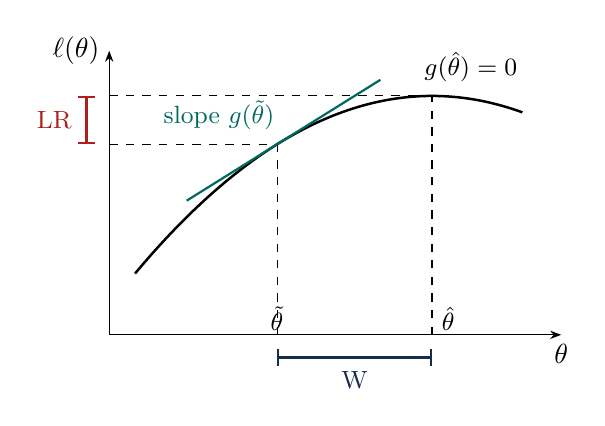
\begin{tikzpicture}[scale=0.82]
 \draw[-{Stealth[length=4pt]}] (0,0) -- (7,0) node[below] {$\theta$};
 \draw[-{Stealth[length=4pt]}] (0,0) -- (0,4.4) node[left] {$\ell(\theta)$};
 \draw[line width=0.9pt,domain=0.4:6.4,samples=60,smooth] plot (\x,{3.7-(\x-5)^2*0.13});
 \draw[dashed] (0,3.7) -- (5,3.7);
 \draw[dashed] (0,2.9512) -- (2.6,2.9512);
 \draw[dashed] (2.6,0) -- (2.6,2.9512);
 \draw[dashed] (5,0) -- (5,3.7);
 \draw[thick,intu] (1.2,{2.9512+0.624*(1.2-2.6)}) -- (4.2,{2.9512+0.624*(4.2-2.6)});
 \node[font=\small,intu] at (1.7,3.4) {slope $g(\tth)$};
 \node[font=\small] at (5.6,4.15) {$g(\hth)=0$};
 \draw[|-|,thick,flagred] (-0.35,2.9512) -- (-0.35,3.7);
 \node[font=\small,flagred] at (-0.85,3.33) {LR};
 \draw[|-|,thick,navy] (2.6,-0.35) -- (5,-0.35);
 \node[font=\small,navy] at (3.8,-0.7) {W};
 \node[font=\small] at (2.6,0.25) {$\tth$};
 \node[font=\small] at (5.25,0.25) {$\hth$};
\end{tikzpicture}
\end{column}
\begin{column}{0.46\textwidth}
\small
\begin{itemize}
 \item \textbf{Wald}: horizontal distance $\hth-\tth$. Needs only $\hth$.
 \item \textbf{LR}: vertical distance $\ell(\hth)-\ell(\tth)$. Needs both.
 \item \textbf{LM} (score): slope $g(\tth)$, the same as $g(\tth)-g(\hth)$ since $g(\hth)=0$. Needs only $\tth$.
\end{itemize}
\end{column}
\end{columns}
\intuition{If $H_{0}$ is true all three distances are small. The question is what units to measure them in (next slide).}
\end{frame}

\begin{frame}{Each distance is measured in units of the information matrix}
Simple null $H_{0}\colon\theta=\thz$ ($r=k$), so $\tth=\thz$:
\begin{align*}
 W&=(\hth-\thz)'\,\In(\hth)\,(\hth-\thz)=n(\hth-\thz)'\Bigl[\frac{-H(\hth)}{n}\Bigr](\hth-\thz)\\
 LM&=g(\tth)'\,\In(\tth)^{-1}g(\tth)=g(\tth)'\bigl[-H(\tth)\bigr]^{-1}g(\tth)\\
 LR&=2\bigl[\ell(\hth)-\ell(\tth)\bigr]
\end{align*}
All three are $\asim\chi^{2}_{r}$ under $H_{0}$. For general restrictions $r(\theta)=0$ (\emph{added}):
$\ W=r(\hth)'\bigl[\hat R\,\In(\hth)^{-1}\hat R'\bigr]^{-1}r(\hth)$.
\flag{MLE III's handout puts $1/n$ next to the full-sample $H$ in LM and drops the $n$ in W. The versions here are consistent with $H=\sum_{t}$ (as in the transcription of MLE III).}
\intuition{Each is ``distance$^{2}$ / variance''. A big slope or a big gap only counts as evidence relative to how noisy it is.}
\end{frame}

\begin{frame}{Why each statistic is $\chi^{2}$ (added)}
Rule used throughout: $z\asim N(0,V)$ with $z$ of length $r$ $\ \Longrightarrow\ z'V^{-1}z\asim\chi^{2}_{r}$.
\begin{align*}
 \text{W:}&\quad \sqrt n(\hth-\thz)\asim N(0,\cI^{-1}) \why{Section 3}\\
 &\quad\Rightarrow\ n(\hth-\thz)'\cI(\hth-\thz)=(\hth-\thz)'\In(\hth-\thz)\asim\chi^{2}_{k}\\
 \text{LM:}&\quad g(\thz)/\sqrt n\asim N(0,\cI) \why{Steps 3--5}\\
 &\quad\Rightarrow\ \tfrac1n g'\cI^{-1}g=g'\In^{-1}g\asim\chi^{2}_{k}\\
 \text{LR:}&\quad \ell(\tth)\approx\ell(\hth)+\tfrac12(\tth-\hth)'H(\tth-\hth) \why{Taylor around $\hth$, where $g(\hth)=0$}\\
 &\quad\Rightarrow\ LR\approx(\hth-\tth)'(-H)(\hth-\tth)\approx W
\end{align*}
\intuition{All three are the same quadratic form to first order, so they share the same $\chi^{2}$ limit.}
\end{frame}

\bridge{Open question: where does $\tth$ come from, and why $\chi^{2}_{r}$ when $r<k$?}
{W, LR and LM, each a squared distance scaled by the information.}
{Restricted ML as a Lagrangian problem. Linearising its first-order conditions gives the variance of $\tth$, the variance of the multipliers, and LM as a test that the multipliers are zero.}

% =====================================================================
\section{8 LM from restricted ML}

\begin{frame}{Restricted ML is a Lagrangian problem}
Maximise $\ell(\theta)$ subject to $r\le k$ restrictions $r(\theta)=0$ (linear case: $R\theta=q$).
\[ \mathcal L(\theta,\lambda)=\ell(\theta)-r(\theta)'\lambda,\qquad
 \underset{r\times k}{R(\theta)}=\frac{\partial r}{\partial\theta'}=
 \begin{bmatrix}\partial r_{1}/\partial\theta_{1}&\cdots&\partial r_{1}/\partial\theta_{k}\\ \vdots&&\vdots\\ \partial r_{r}/\partial\theta_{1}&\cdots&\partial r_{r}/\partial\theta_{k}\end{bmatrix} \]
First-order conditions ($k+r$ equations):
\[ g(\tth)-R(\tth)'\tilde\lambda=0\quad(k\times1),\qquad r(\tth)=0\quad(r\times1). \]
\intuition{$\tilde\lambda$ is the shadow price of the restrictions. If $H_{0}$ is true, imposing it costs little likelihood, so $\tilde\lambda\approx0$.}
\end{frame}

\begin{frame}{Linearising the FOC gives one linear system for $(\tth,\tilde\lambda)$}
\begin{align*}
 g(\thz)+H(\bar\theta)(\tth-\thz)-R'\tilde\lambda&=0 \why{expand $g(\tth)$ around $\thz$}\\
 R\,(\tth-\thz)&=0 \why{$r(\tth)=r(\thz)=0$ under $H_{0}$, mean value}
\end{align*}
Stack them, then scale ($H/n$, $\sqrt n(\tth-\thz)$, $\tilde\lambda/\sqrt n$, $g/\sqrt n$; each row is just multiplied by $1/\sqrt n$):
\[ \begin{bmatrix}-H&R'\\ R&0\end{bmatrix}\!\begin{bmatrix}\tth-\thz\\ \tilde\lambda\end{bmatrix}=\begin{bmatrix}g(\thz)\\0\end{bmatrix}
 \ \Longrightarrow\
 \underbrace{\begin{bmatrix}\cI&R'\\ R&0\end{bmatrix}}_{M}\!\begin{bmatrix}\sqrt n(\tth-\thz)\\ \tilde\lambda/\sqrt n\end{bmatrix}\aeq\begin{bmatrix}g(\thz)/\sqrt n\\0\end{bmatrix} \]
using $-H/n\to-\cH=\cI$ (IM equality) and $R(\bar\theta)\to R(\thz)$ (consistency). $M$ is $(k+r)\times(k+r)$.
\intuition{It is the Step 1--2 argument of Section 3, with $r$ extra rows for the constraints.}
\end{frame}

\begin{frame}{Inverting the bordered matrix gives both variances}
With $S=R\,\cI^{-1}R'$ ($r\times r$), the partitioned inverse is
\[ M^{-1}=\begin{bmatrix}\cI^{-1}-\cI^{-1}R'S^{-1}R\,\cI^{-1} & \cI^{-1}R'S^{-1}\\[4pt] S^{-1}R\,\cI^{-1} & -S^{-1}\end{bmatrix}. \]
Since $g/\sqrt n\asim N(0,\cI)$, the solution has variance $M^{-1}\begin{bmatrix}\cI&0\\0&0\end{bmatrix}M^{-1\prime}$. Multiplying out:
\begin{align*}
 \Var\bigl(\sqrt n(\tth-\thz)\bigr)&=\cI^{-1}-\cI^{-1}R'S^{-1}R\,\cI^{-1}\\
 \Var\bigl(\tilde\lambda/\sqrt n\bigr)&=S^{-1}R\,\cI^{-1}\,\cI\,\cI^{-1}R'S^{-1}=S^{-1}=\bigl(R\,\cI^{-1}R'\bigr)^{-1}
\end{align*}
\flag{MLE IV (10) is written in $\cH$; its bottom-right block $-(R\cH^{-1}R')^{-1}$ should be $+(R\cH^{-1}R')^{-1}$. This does not affect the variances, because the zero rows of the middle matrix remove that block.}
\intuition{Only the first block column of $M^{-1}$ matters, because the randomness enters only through $g$.}
\end{frame}

\begin{frame}{The variance gap $\Var(\hth)-\Var(\tth)$ is p.s.d.: restrictions buy precision}
\begin{align*}
 \Var\bigl(\sqrt n(\hth-\thz)\bigr)-\Var\bigl(\sqrt n(\tth-\thz)\bigr)
 &=\cI^{-1}-\bigl[\cI^{-1}-\cI^{-1}R'S^{-1}R\,\cI^{-1}\bigr]\\
 &=A'S^{-1}A,\qquad A=R\,\cI^{-1}\ (r\times k)
\end{align*}
For any $c$: $\ c'A'S^{-1}Ac=(Ac)'S^{-1}(Ac)\ge0$, because $S^{-1}$ is positive definite. The gap is p.s.d.\ with rank $r$.

\vspace{4pt}
Linear model, restricted LS $b^{*}$ (Lesson 6):
\[ \Var(b)-\Var(b^{*})=\sigma^{2}(X'X)^{-1}R'\bigl(R(X'X)^{-1}R'\bigr)^{-1}R(X'X)^{-1}. \]
\intuition{Imposing true restrictions removes noise in $r$ directions. This gap reappears as the Hausman variance in Section 10.}
\end{frame}

\begin{frame}{LM tests whether the shadow prices are zero; it equals the score form}
\begin{align*}
 \frac{\tilde\lambda}{\sqrt n}&\asim N\bigl(0,S^{-1}\bigr)
 \ \Longrightarrow\ \Bigl(\frac{\tilde\lambda}{\sqrt n}\Bigr)'S\Bigl(\frac{\tilde\lambda}{\sqrt n}\Bigr)=\frac1n\tilde\lambda'R\,\cI^{-1}R'\tilde\lambda\asim\chi^{2}_{r}\\
 g(\tth)&=R'\tilde\lambda \why{FOC}\\
 \Longrightarrow\ LM&=\frac1n\,\tilde g'\,\cI^{-1}\,\tilde g=\tilde g'\,\In(\tth)^{-1}\tilde g\ \asim\ \chi^{2}_{r},\qquad\tilde g=g(\tth)
\end{align*}
\begin{itemize}
 \item Why $r$ degrees of freedom and not $k$: $\tilde g=R'\tilde\lambda$ lies in the $r$-dimensional column space of $R'$.
 \item In practice use the score form: $\tilde g$ is easy to compute, $\tilde\lambda$ often is not.
\end{itemize}
\flag{MLE IV (15) is printed $g(\tth)=-R'\tilde\lambda$. The FOC gives $+$; the sign does not affect the quadratic form.}
\intuition{The $\lambda$ form shows \emph{why} the statistic is $\chi^{2}_{r}$; the score form is the one you compute.}
\end{frame}

\begin{frame}{Three interchangeable LM versions; the OPG one is a regression}
\[ LM_{\cI}=\tilde g'\,\In(\tth)^{-1}\tilde g,\qquad
   LM_{H}=-\tilde g'\,\tilde H^{-1}\tilde g,\qquad
   LM_{OPG}=\tilde g'(\tilde G'\tilde G)^{-1}\tilde g . \]
All are asymptotically equivalent ($\tilde H=H(\tth)$, $\tilde G=G(\tth)$, full-sample, so no $1/n$). For OPG, use $\tilde g=\tilde G'\iota$:
\[ LM_{OPG}=\iota'\tilde G(\tilde G'\tilde G)^{-1}\tilde G'\iota
 =\text{ESS from the regression}\ \ \iota=\tilde G\,b+\text{errors}. \]
\begin{itemize}
 \item Since $\iota'\iota=n$: $\ LM_{OPG}=n-\mathrm{SSR}=nR^{2}_{u}$ (uncentred $R^{2}$).
 \item The minus sign in $LM_{H}$ is needed because $H$ is negative definite.
\end{itemize}
\intuition{Same OPG regression as in Section 4, but at $\tth$. There $\hat g=0$ made $b=0$; here $\tilde g\neq0$, and how much it explains is the test.}
\end{frame}

\bridge{Open question: in a model we know, are W, LR and LM equal?}
{LM $=\tilde g'\In^{-1}\tilde g\asim\chi^{2}_{r}$, and W and LR have the same limit.}
{Compute all three exactly in the normal linear model with $H_{0}\colon\beta_{1}=0$. They are \emph{not} equal in finite samples, and they are always ordered.}

% =====================================================================
\section{9 W, LR, LM in the linear model}

\begin{frame}{Set-up: test $\beta_{1}=0$ in $y=X_{1}\beta_{1}+X_{2}\beta_{2}+u$}
$X=[X_{1}\ X_{2}]$ ($n\times k_{1}$, $n\times k_{2}$), $u\sim N(0,\sigma^{2}I)$, $M_{i}=I-X_{i}(X_{i}'X_{i})^{-1}X_{i}'$.
\begin{itemize}
 \item Unrestricted: OLS $b_{1}=(X_{1}'M_{2}X_{1})^{-1}X_{1}'M_{2}y$ (FWL), $\hat u$, $\ \hat\sigma^{2}=\hat u'\hat u/n=\mathrm{USSR}/n$.
 \item Restricted: $\tilde\beta_{2}=(X_{2}'X_{2})^{-1}X_{2}'y$, $\ \tilde u=y-X_{2}\tilde\beta_{2}=M_{2}y$, $\ \tilde\sigma^{2}=\mathrm{RSSR}/n$.
\end{itemize}
Score at the restricted estimate:
\[ g_{\beta}(\tth)=\frac{1}{\tilde\sigma^{2}}\begin{bmatrix}X_{1}'\tilde u\\ X_{2}'\tilde u\end{bmatrix}
 =\frac{1}{\tilde\sigma^{2}}\begin{bmatrix}X_{1}'M_{2}y\\ 0\end{bmatrix}
 \begin{matrix}(k_{1}\times1)\\(k_{2}\times1)\end{matrix},
 \qquad g_{\sigma^{2}}(\tth)=0 . \]
($X_{2}'M_{2}=0$; and $\tilde\sigma^{2}$ solves its own FOC.)
\intuition{At $\tth$ the score is zero in every direction that was free. It is nonzero only in the restricted direction $\beta_{1}$.}
\end{frame}

\begin{frame}{LM uses only the top-left block of $(X'X)^{-1}$}
$\In$ is block-diagonal and $g_{\sigma^{2}}(\tth)=0$, so only the $\beta$ block enters: $\ LM=g_{\beta}'\bigl[\tilde\sigma^{2}(X'X)^{-1}\bigr]g_{\beta}$. By the partitioned inverse,
\[ (X'X)^{-1}=\begin{bmatrix}(X_{1}'M_{2}X_{1})^{-1} & \ast\\ \ast & (X_{2}'M_{1}X_{2})^{-1}\end{bmatrix}. \]
Since the second block of $g_{\beta}$ is zero, only the top-left block multiplies nonzero entries:
\begin{align*}
 LM&=\frac{1}{\tilde\sigma^{4}}\cdot\tilde\sigma^{2}\cdot y'M_{2}X_{1}(X_{1}'M_{2}X_{1})^{-1}X_{1}'M_{2}y=\frac{Q}{\tilde\sigma^{2}},\\
 Q&\equiv y'M_{2}X_{1}(X_{1}'M_{2}X_{1})^{-1}X_{1}'M_{2}y .
\end{align*}
\intuition{$Q$ is how much $X_{1}$ explains of $y$ after $X_{2}$ has been partialled out.}
\end{frame}

\begin{frame}{W and LR in the same model: all three are functions of RSSR and USSR}
\begin{align*}
 W&=b_{1}'\bigl[\hat\sigma^{2}(X_{1}'M_{2}X_{1})^{-1}\bigr]^{-1}b_{1}=\frac{Q}{\hat\sigma^{2}}
   \why{substitute $b_{1}$}\\
 LR&=2\bigl[\ell^{c}(\hth)-\ell^{c}(\tth)\bigr]=n\log\frac{\mathrm{RSSR}}{\mathrm{USSR}}
   \why{$\ell^{c}=-\tfrac n2\log\mathrm{SSR}+$const}\\
 \mathrm{RSSR}-\mathrm{USSR}&=Q \why{FWL}
\end{align*}
\begin{itemize}
 \item W and LM are the \emph{same} quadratic form $Q$, divided by $\hat\sigma^{2}$ (unrestricted) versus $\tilde\sigma^{2}$ (restricted).
 \item Since $\tilde\sigma^{2}\ge\hat\sigma^{2}$, already $LM\le W$.
\end{itemize}
\intuition{The tests differ only in which variance estimate they use and whether they take a log.}
\end{frame}

\begin{frame}{Write all three in one number: $a=\mathrm{RSSR}/\mathrm{USSR}\ge1$}
\begin{align*}
 W&=\frac{Q}{\hat\sigma^{2}}=\frac{n(\mathrm{RSSR}-\mathrm{USSR})}{\mathrm{USSR}}=n\,(a-1)\\
 LR&=n\log a\\
 LM&=\frac{Q}{\tilde\sigma^{2}}=\frac{n(\mathrm{RSSR}-\mathrm{USSR})}{\mathrm{RSSR}}=n\Bigl(1-\frac1a\Bigr)
\end{align*}
$a\ge1$ because adding the restriction can never lower the SSR.
\intuition{The whole comparison reduces to three functions of one number $a$. The ordering of the tests is then the ordering of these functions.}
\end{frame}

\begin{frame}{The gaps $W-LR$ and $LR-LM$ are never negative}
\begin{columns}[c,onlytextwidth]
\begin{column}{0.56\textwidth}
\small
\begin{align*}
 W-LR&=n\bigl[(a-1)-\log a\bigr]\ \ge0\\
 LR-LM&=n\bigl[\log a-(1-\tfrac1a)\bigr]\ \ge0
\end{align*}
\begin{itemize}
 \item $\log a\le a-1$: $\log$ is concave, so it lies below its tangent at $a=1$.
 \item Apply that to $1/a$: $\log\frac1a\le\frac1a-1$, i.e.\ $\log a\ge1-\frac1a$.
 \item Equality only at $a=1$. \ So $\ \boxed{W\ge LR\ge LM}\ $ in every sample.
\end{itemize}
\end{column}
\begin{column}{0.42\textwidth}
\centering
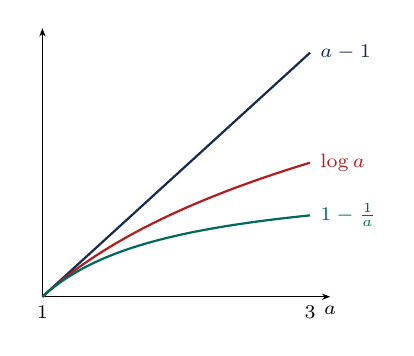
\begin{tikzpicture}[xscale=1.7,yscale=1.55]
 \draw[-{Stealth[length=3pt]}] (1,0) -- (3.15,0) node[below] {\scriptsize $a$};
 \draw[-{Stealth[length=3pt]}] (1,0) -- (1,2.2);
 \node[below,font=\scriptsize] at (1,0) {1};
 \node[below,font=\scriptsize] at (3,0) {3};
 \draw[thick,navy,domain=1:3,samples=40] plot (\x,{\x-1}) node[right,font=\scriptsize] {$a-1$};
 \draw[thick,flagred,domain=1:3,samples=40] plot (\x,{ln(\x)}) node[right,font=\scriptsize] {$\log a$};
 \draw[thick,intu,domain=1:3,samples=40] plot (\x,{1-1/\x}) node[right,font=\scriptsize] {$1-\frac1a$};
\end{tikzpicture}
\end{column}
\end{columns}
\flag{the handout gets $LR>LM$ from $LR\approx a\cdot LM$ (approximate); the argument here is exact. Its reference ``Evans and Savin (1980)'' may be 1982.}
\intuition{One concave function sandwiched between two others gives the whole ordering.}
\end{frame}

\begin{frame}{Asymptotically the gaps vanish, but in finite samples the tests can conflict}
Under $H_{0}$, $W=n(a-1)=O_{p}(1)$, so $a-1=O_{p}(1/n)$. Expand $\log a=(a-1)-\frac{(a-1)^{2}}{2}+\cdots$:
\[ W-LR=n\,\frac{(a-1)^{2}}{2}+\cdots=\frac{W^{2}}{2n}+\cdots\ \longrightarrow\ 0 \]
and similarly $LR-LM\to0$. So all three $\asim\chi^{2}_{k_{1}}$.
\begin{itemize}
 \item In a finite sample, with critical value $c$, it can happen that $LM<c<W$: LM accepts while W rejects.
 \item For small $n$, none of the three has exactly a $\chi^{2}$ distribution.
\end{itemize}
\intuition{Same limit, different finite-sample sizes. W rejects most often and LM least often.}
\end{frame}

\bridge{Open question: can we test a model by comparing two \emph{different} estimators?}
{W, LR and LM compare restricted and unrestricted ML within one model.}
{Hausman: compare an estimator that is efficient under $H_{0}$ with one that stays consistent when $H_{0}$ fails. The key is a variance \emph{difference}.}

% =====================================================================
\section{10 Hausman test}

\begin{frame}{Hausman: compare an efficient estimator with a robust one}
\begin{itemize}
 \item $\tth$: consistent and asymptotically \textbf{efficient under $H_{0}$}; inconsistent if $H_{0}$ fails.
 \item $\hth$: consistent whether or not $H_{0}$ holds, but \textbf{not efficient} under $H_{0}$.
\end{itemize}
\[ H_{0}\text{ true: }\plim(\hth-\tth)=0,\qquad H_{0}\text{ false: }\plim(\hth-\tth)\neq0 . \]
Build a test on the contrast $\hat q=\hth-\tth$. We need $\Var(\hat q)$.
\intuition{If the efficient estimator and the safe estimator disagree by more than noise, the assumptions that make the efficient one valid are suspect.}
\end{frame}

\begin{frame}{Key result: the variance of the contrast is a difference, not a sum}
In general $\ \Var(\hth-\tth)=\Var\hth+\Var\tth-2\Cov(\hth,\tth)$. \textbf{Claim:} $\Cov(\hth,\tth)=\Var(\tth)$ under $H_{0}$, so
$\ \boxed{\Var(\hth-\tth)=\Var(\hth)-\Var(\tth)}$.

\smallskip
\textbf{Proof} (scalar). $\theta^{*}(w)=\tth+w(\hth-\tth)$ is consistent for every $w$. With $V_{0}=\Var\tth$, $V_{1}=\Var\hth$, $C=\Cov$:
\begin{align*}
 \Var\theta^{*}(w)&=(1-w)^{2}V_{0}+w^{2}V_{1}+2w(1-w)C\\
 \frac{d}{dw}\Var\theta^{*}\Big|_{w=0}&=-2V_{0}+2C
   \why{$\tth$ efficient $\Rightarrow$ $w=0$ is the minimum, so this is $0$}
\end{align*}
Hence $C=V_{0}$. Gap form: $\Cov(\tth,\hth-\tth)=C-V_{0}=0$. (Vector case: the same argument for $c'\theta^{*}$ with $\theta^{*}=\tth+wA(\hth-\tth)$, for all $c$ and $A$.)
\flag{MLE V's derivative is printed with $+2(1-\lambda)\Var(\tth)$; differentiating $(1-w)^{2}$ gives $-2(1-w)$.}
\intuition{If the efficient estimator were correlated with $\hth-\tth$, we could mix in some $\hth$ and do better, which contradicts efficiency.}
\end{frame}

\begin{frame}{The Hausman statistic is $\chi^{2}$ with $r$ (not $k$) degrees of freedom}
\[ \mathcal{W}_{H}=(\hth-\tth)'\bigl[\Var(\hth)-\Var(\tth)\bigr]^{-}(\hth-\tth)\ \asim\ \chi^{2}_{r} \]
For ML, plug in the variance gap of Section 8 (evaluated at $\tth$):
\[ \Var(\hth)-\Var(\tth)=\frac1n\,\cI^{-1}R'\bigl(R\,\cI^{-1}R'\bigr)^{-1}R\,\cI^{-1}
   \qquad(k\times k,\ \text{rank } r). \]
\begin{itemize}
 \item Singular when $r<k$: hence the generalised inverse $^{-}$ and $r$ degrees of freedom.
 \item Automatically p.s.d.: it equals $\Var(\hth-\tth)$, and a variance cannot be negative.
\end{itemize}
\flag{MLE V writes an ordinary inverse in (4) and $[R\,\cI\,R']^{-1}$ inside $\Var(\tth)$; the deck uses $^{-}$ and $[R\,\cI^{-1}R']^{-1}$ (as in MLE IV).}
\intuition{The contrast can only move in the $r$ directions the restrictions affect, so only $r$ independent pieces of evidence exist.}
\end{frame}

\begin{frame}{In the linear model, Hausman reproduces the Wald test}
OLS $b$ and restricted LS $b^{*}$ for $R\beta=q$, with $S=R(X'X)^{-1}R'$:
\begin{align*}
 b-b^{*}&=(X'X)^{-1}R'S^{-1}(Rb-q)\\
 \Var(b)-\Var(b^{*})&=\sigma^{2}P,\qquad P=(X'X)^{-1}R'S^{-1}R(X'X)^{-1}
\end{align*}
$X'X$ is a generalised inverse of $P$ ($P\,X'X\,P=P$; the $S$'s cancel). Hence
\begin{align*}
 \frac{1}{\sigma^{2}}(b-b^{*})'X'X(b-b^{*})
 &=\frac{1}{\sigma^{2}}(Rb-q)'S^{-1}\underbrace{R(X'X)^{-1}X'X(X'X)^{-1}R'}_{=S}S^{-1}(Rb-q)\\
 &=\frac{1}{\sigma^{2}}(Rb-q)'\bigl(R(X'X)^{-1}R'\bigr)^{-1}(Rb-q)\ \sim\ \chi^{2}_{r},
\end{align*}
which is the Wald statistic ($r$ times $F$ once $s^{2}$ replaces $\sigma^{2}$).
\intuition{When the two estimators are restricted and unrestricted ML, Hausman is nothing new. Its value is for other efficient/robust pairs (e.g.\ OLS versus IV).}
\end{frame}

\bridge{Open question: can LM be computed without deriving $\In^{-1}$ by hand?}
{LM $=\tilde g'\In^{-1}\tilde g$; Hausman for estimator comparisons.}
{When the model is a regression with normal errors, LM is the explained sum of squares, i.e.\ $nR^{2}$, of an OLS regression. Example: testing for AR(1) errors.}

% =====================================================================
\section{11 LM by artificial regression}

\begin{frame}{Write a regression with AR(1) errors as a nonlinear regression}
$y_{t}=X_{t}\beta+u_{t}$, $\ u_{t}=\rho u_{t-1}+\varepsilon_{t}$, $\ \varepsilon_{t}\sim$ iid $N(0,\sigma^{2})$. Substitute $u_{t-1}=y_{t-1}-X_{t-1}\beta$:
\[ y_{t}=\underbrace{\rho y_{t-1}+X_{t}\beta-\rho X_{t-1}\beta}_{f_{t}(\alpha)}+\varepsilon_{t},
   \qquad \alpha=\begin{bmatrix}\beta\\ \rho\end{bmatrix}\ \ (p\times1,\ p=k+1). \]
Derivatives of the regression function, one row per observation:
\[ \underset{n\times p}{F(\alpha)}=
 \begin{bmatrix}
  \partial f_{1}/\partial\alpha_{1} & \cdots & \partial f_{1}/\partial\alpha_{p}\\
  \vdots & \ddots & \vdots\\
  \partial f_{n}/\partial\alpha_{1} & \cdots & \partial f_{n}/\partial\alpha_{p}
 \end{bmatrix},\qquad F_{ti}=\frac{\partial f_{t}(\alpha)}{\partial\alpha_{i}} . \]
\intuition{Once the model is ``$y=f(\alpha)+$ normal error'', Section 5's results apply with $X$ replaced by $F$.}
\end{frame}

\begin{frame}{Score and information have the regression form}
\[ \ell(\alpha,\sigma)=\text{const}-n\log\sigma-\frac{1}{2\sigma^{2}}\sum_{t}\bigl(y_{t}-f_{t}(\alpha)\bigr)^{2} \]
\begin{align*}
 g_{\alpha}&=\frac{1}{\sigma^{2}}F'(\alpha)\bigl(y-f(\alpha)\bigr)\ \ (p\times1),
 &g_{\sigma}&=-\frac n\sigma+\frac{1}{\sigma^{3}}\textstyle\sum_{t}\bigl(y_{t}-f_{t}\bigr)^{2}\\
 \In&=\begin{bmatrix}\dfrac{F'F}{\sigma^{2}}&0\\[6pt]0&\dfrac{2n}{\sigma^{2}}\end{bmatrix},
 &\In^{-1}&=\begin{bmatrix}\sigma^{2}(F'F)^{-1}&0\\[4pt]0&\dfrac{\sigma^{2}}{2n}\end{bmatrix}
\end{align*}
(Off-diagonal zero because $\E\varepsilon_{t}=0$; the $\sigma$ entry is $-\frac{n}{\sigma^{2}}+\frac{3n\sigma^{2}}{\sigma^{4}}=\frac{2n}{\sigma^{2}}$.)
\flag{MLE V prints the lower-right block of $\In^{-1}$ as $2n/\sigma^{2}$; the inverse is $\sigma^{2}/(2n)$. MLE V calls the log-likelihood $L$; here it is $\ell$.}
\intuition{Exactly the normal-linear-model structure of Section 5, now in the $\sigma$ parametrisation.}
\end{frame}

\begin{frame}{LM is the explained sum of squares of an artificial regression}
$H_{0}$ imposes $r$ restrictions on $\alpha$; restricted ML $\tth=(\tilde\alpha,\tilde\sigma)$, $\tilde f=f(\tilde\alpha)$, $\tilde F=F(\tilde\alpha)$.
\begin{align*}
 LM&=\tilde g_{\alpha}'\,\bigl[\tilde\sigma^{2}(\tilde F'\tilde F)^{-1}\bigr]\,\tilde g_{\alpha}
   \why{block-diagonal $\In$, and $g_{\sigma}(\tth)=0$}\\
 &=\frac{1}{\tilde\sigma^{2}}(y-\tilde f)'\tilde F\cdot\tilde\sigma^{2}(\tilde F'\tilde F)^{-1}\cdot\frac{1}{\tilde\sigma^{2}}\tilde F'(y-\tilde f)\\
 &=\frac{1}{\tilde\sigma^{2}}(y-\tilde f)'\tilde F(\tilde F'\tilde F)^{-1}\tilde F'(y-\tilde f)
\end{align*}
This is $z'P_{\tilde F}z$ with $z=(y-\tilde f)/\tilde\sigma$, i.e.\ the \textbf{ESS} from the regression
$\ \dfrac{y-\tilde f}{\tilde\sigma}=\tilde F\,b+\text{errors}$.

\smallskip
(Recall: in $y=X\beta+u$, $\ \mathrm{ESS}=b'X'Xb=y'X(X'X)^{-1}X'y$.)
\intuition{Regress the restricted residuals on the derivatives of the regression function. If they explain a lot, the restrictions are binding.}
\end{frame}

\begin{frame}{Because the regressand has TSS $=n$, LM $=nR^{2}$}
\begin{align*}
 \mathrm{TSS}&=\frac{(y-\tilde f)'(y-\tilde f)}{\tilde\sigma^{2}}=n
   \why{$\tilde\sigma^{2}=(y-\tilde f)'(y-\tilde f)/n$}\\
 \mathrm{RSS}&=\mathrm{TSS}-\mathrm{ESS}=n-LM\\
 R^{2}&=\frac{\mathrm{ESS}}{\mathrm{TSS}}=\frac{LM}{n}
 \qquad\Longrightarrow\qquad \boxed{\,LM=nR^{2}\ \asim\ \chi^{2}_{r}\,}
\end{align*}
$R^{2}$ is the \textbf{uncentred} $R^{2}$. It does not change if the regressand is not divided by $\tilde\sigma$, because $R^{2}$ is scale-invariant.
\intuition{Dividing by $\tilde\sigma$ makes the regressand have ``sum of squares $n$''. The share explained, times $n$, is the test.}
\end{frame}

\begin{frame}{Testing for AR(1) errors: regress OLS residuals on $X_{t}$ and $e_{t-1}$}
Under $H_{0}\colon\rho=0$: $\tilde\alpha=(\tilde\beta,0)$, $\tilde\beta=$ OLS, $\tilde f_{t}=X_{t}\tilde\beta$, $e_{t}=y_{t}-X_{t}\tilde\beta$. Derivatives at $\tilde\alpha$:
\[ F_{t\beta_{i}}=X_{ti}-\rho X_{t-1,i}\ \xrightarrow{\ \rho=0\ }\ X_{ti},\qquad
   F_{t\rho}=y_{t-1}-X_{t-1}\beta\ \xrightarrow{\ \tilde\beta\ }\ e_{t-1}. \]
\textbf{Step 1.} OLS of $y_{t}$ on $X_{t}$; keep the residuals $e_{t}$.\quad
\textbf{Step 2.} Regress $e_{t}$ on $X_{t}$ and $e_{t-1}$: $\ nR^{2}\asim\chi^{2}_{1}$ (or the $t$-statistic on $e_{t-1}$).
\begin{itemize}\footnotesize
 \item Regressors are $X_{t}$ themselves (the derivative), not $X_{t}\tilde\beta$. With a constant in $X$, centred $=$ uncentred $R^{2}$.
 \item $e_{0}$: set it to $0$ or drop $t=1$ (asymptotically irrelevant).
 \item AR($p$) (\emph{added}): add $e_{t-1},\dots,e_{t-p}$; $\ nR^{2}\asim\chi^{2}_{p}$.
 \item Versus the GNR test (Lesson 13): same regressors, but read with $t$/$F$ (re-estimated $\sigma^{2}$); LM uses $\tilde\sigma^{2}$. Asymptotically equivalent.
\end{itemize}
\intuition{If last period's residual helps predict this period's residual, beyond what $X_{t}$ explains, the errors are autocorrelated.}
\end{frame}

% =====================================================================
\section{Summary}

\begin{frame}{Summary: the whole chain on one slide}
\footnotesize
\renewcommand{\arraystretch}{1.3}
\begin{tabular}{@{}lll@{}}
 \textbf{object} & \textbf{formula} & \textbf{key fact}\\ \hline
 log-likelihood & $\ell=\sum_{t}\ell_{t}$ (scalar) & independence $\Rightarrow$ a sum\\
 score & $g=\partial\ell/\partial\theta=G'\iota$ ($k\times1$) & $\E g(\thz)=0$\\
 FOC $\to$ estimator & $g(\hth)=0$ & invariant, consistent, biased in finite $n$\\
 Hessian & $H=\partial^{2}\ell/\partial\theta\partial\theta'$ ($k\times k$) & curvature; $H/n\to\cH$\\
 information & $\In=\E(gg')=\E(G'G)$ ($k\times k$) & $=-\E H$ \textbf{if the model is correct}\\
 asymptotic variance & $\Var(\hth)\approx\In^{-1}$ & else sandwich $\cH^{-1}\cI\cH^{-1}/n$\\
 estimators of $\Var$ & $\In(\hth)^{-1}$, $(-\hat H)^{-1}$, $(\hat G'\hat G)^{-1}$ & equal asymptotically\\
 tests & W, LR, LM $\asim\chi^{2}_{r}$ & LM $=\tilde g'\In^{-1}\tilde g$, from $\tilde\lambda$\\
 Hausman & $(\hth-\tth)'[\Var\hth-\Var\tth]^{-}(\hth-\tth)$ & $\Var$(contrast) $=$ difference\\
 by regression & LM $=$ ESS $=nR^{2}$ & AR(1): $e_{t}$ on $X_{t},e_{t-1}$
\end{tabular}

\vspace{4pt}
\textbf{Linear model:} $b=(X'X)^{-1}X'y$, $\ \Var(b)=\sigma^{2}(X'X)^{-1}$, $\ \hat\sigma^{2}=e'e/n$, $\ \In=\mathrm{diag}\bigl(X'X/\sigma^{2},\,n/2\sigma^{4}\bigr)$, $\ W\ge LR\ge LM$.
\end{frame}

\begin{frame}{Common exam traps}
\footnotesize
\begin{columns}[T,onlytextwidth]
\begin{column}{0.5\textwidth}
\begin{enumerate}
 \item $G_{t}'G_{t}$ is $k\times k$; $G_{t}G_{t}'$ is a scalar.
 \item Total $\In$ vs.\ average $\cI$: a factor of $n$. LM $=\tilde g'\In^{-1}\tilde g=\frac1n\tilde g'\cI^{-1}\tilde g$; W carries an $n$ with $\cI$.
 \item $H$ is negative definite: $\Var=(-H)^{-1}$, and the Hessian LM needs a minus sign.
 \item $\cH=-\cI$ needs a \textbf{correct model}. Otherwise use the sandwich.
 \item ML $\hat\sigma^{2}=e'e/n$ is biased; $s^{2}$ uses $n-k$.
 \item ML is generally biased (invariance + Jensen), but asymptotically efficient.
 \item Parametrisation: info for $\sigma^{2}$ is $n/2\sigma^{4}$, for $\sigma$ it is $2n/\sigma^{2}$. Invert: $2\sigma^{4}/n$, $\sigma^{2}/2n$.
\end{enumerate}
\end{column}
\begin{column}{0.5\textwidth}
\begin{enumerate}\setcounter{enumi}{7}
 \item Cram\'er--Rao bound is $\In^{-1}=(n\cI)^{-1}$, not $\cI^{-1}$.
 \item W uses $\hat\sigma^{2}$ (unrestricted), LM uses $\tilde\sigma^{2}$ (restricted). Hence $W\ge LR\ge LM$, every sample.
 \item Degrees of freedom $=$ number of restrictions $r$, not $k$ (LM and Hausman).
 \item Hausman: the variance of the contrast is a \emph{difference} (valid only under $H_{0}$ with $\tth$ efficient), and it needs a generalised inverse.
 \item $nR^{2}$ uses the \emph{uncentred} $R^{2}$; the regressors are $X_{t}$, not $X_{t}\tilde\beta$.
 \item Jacobian: transforming $y$ adds $\log|\det J|$ to $\ell$; forgetting it lets SSR $\to0$.
\end{enumerate}
\end{column}
\end{columns}
\end{frame}

\end{document}
